\documentclass{WCCM-ECCOMAS_2026_Full_Paper}

\usepackage{graphicx}
\usepackage{amsmath}
\usepackage{amssymb}
\usepackage{booktabs}
\usepackage{longtable}
\usepackage{xcolor}
\usepackage{float}
% Let a page carry more float and less text before LaTeX defers to a float page,
% so figures settle near their reference instead of queueing up at the end.
\renewcommand{\topfraction}{0.90}
\renewcommand{\bottomfraction}{0.75}
\renewcommand{\textfraction}{0.08}
\renewcommand{\floatpagefraction}{0.70}
\setcounter{topnumber}{3}
\setcounter{bottomnumber}{2}
\setcounter{totalnumber}{4}
\usepackage{tikz}
\usetikzlibrary{arrows.meta,positioning,fit,calc}
\usepackage[colorlinks=true,linkcolor=blue,urlcolor=blue,citecolor=blue]{hyperref}

% ---------------------------------------------------------------
% Title --- all caps per ECCOMAS format
% ---------------------------------------------------------------
\title{Spatial Shock-Gated Mixture of Experts for Transonic Surface-Load Prediction}

\author{Marta Arnabat-Mart\'{\i}n$^{*}$, Andr\'{e}s Mateo-Gab\'{\i}n$^{\P}$, Sven A. Lanzan-Ferran$^{\P}$ and Gonzalo Rubio$^{\dag}$}
\shortauthors{Marta Arnabat-Mart\'{\i}n}

\address{%
$^{*}$ Flight Physics Technology and Capability, Airbus Defence and Space,
C/ Aviocar 2, 28906 Getafe, Madrid, Spain; and Universidad Polit\'{e}cnica
de Madrid, Plaza Cardenal Cisneros 3, 28040 Madrid, Spain\\
e-mail: marta.arnabt-martin@airbus.com \\[6pt]
$^{\P}$ Flight Physics Technology and Capability, Airbus Defence and Space,
C/ Aviocar 2, 28906 Getafe, Madrid, Spain\\
e-mail: andres.mateo@airbus.com, sven\_agustin-lanzan@airbus.com \\[6pt]
$^{\dag}$ Applied Mathematics Department, School of Aeronautics, and Center
of Computational Simulation, Universidad Polit\'{e}cnica de Madrid,
28040 Madrid, Spain
}

\keywords{shock capture, mixture of experts, graph neural network,
Gumbel-Softmax routing, physics-informed machine learning, RANS surrogate}

\summary{AeroSurrogate is a physics-aware machine learning surrogate
for the surface coefficients $[C_p, C_{fx}, C_{fy}, C_{fz}]$ on a
transonic transport configuration, requiring no CFD solver at
inference.  An eight-layer message-passing graph neural network over a
$k$-nearest-neighbour graph of the surface maps every node to a latent
read by a shock indicator, a shock-gated Mixture of Experts for $C_p$
and a friction head.  The shock expert adds a residual scaled by the
predicted shock probability, an explicit mechanism for the
discontinuity: ablating it triples the $C_p$ mean absolute error on
shock nodes, from $0.0458$ to $0.1370$.  Shock labels derive from real
RANS pressures via the critical pressure coefficient, not from
isentropic pseudo-labels.  Trained on the ONERA CRM WBPN database and
fine-tuned head-only with the backbone frozen, it reaches
$R^{2}=0.9729$ for $C_p$ and $0.9027$--$0.9209$ for the skin-friction
components over 36\,508\,360 held-out surface points from 140
simulations excluded from model selection.}

\begin{document}
\maketitle

% ================================================================
\section{INTRODUCTION}
% ================================================================

In transonic flight, normal shocks on wing surfaces produce strong
adverse pressure gradients that drive boundary-layer thickening,
separation and buffet onset, and so govern the drag-divergence Mach
number and the structural loads envelope~\cite{Vassberg2008,Levy2013}.
Reynolds-Averaged Navier--Stokes (RANS) solvers resolve that structure
at $\mathcal{O}(10^{3}$--$10^{4})$ CPU-hours per operating condition,
which rules them out of high-frequency pipelines such as shape
optimisation or real-time loads estimation.  Machine learning
surrogates are the practical alternative~\cite{Han2018,Bhatnagar2019},
but a single smooth network trained across subsonic, transonic and
separated regimes learns an interpolant that blurs the shock and
underestimates peak suction, because the smeared solution lowers the
average error over the predominantly smooth remainder of the
surface.

Existing machine learning shock indicators work at the volumetric
field level, from neural troubled-cell indicators~\cite{Ray2018} to
their convolutional successors~\cite{Discacciati2020}.  They require
volumetric data, inaccessible in the surface-only setting of
experimental aerodynamics or flight test, and commonly rely on
pseudo-labels from isentropic assumptions on the inputs, which renders
the problem circular.  Physics-informed neural
networks~\cite{Raissi2019} avoid the pseudo-labels but need the
governing equations embedded explicitly.

This work addresses both gaps with \emph{AeroSurrogate}, a
$4.6\times 10^{6}$-parameter spatial architecture predicting
$[C_p, C_{fx}, C_{fy}, C_{fz}]$ at every mesh node from surface
geometry and flight condition alone: shock detection becomes a
neighbourhood operation on a graph-network latent, the discontinuity
receives a dedicated expert, and the labels come from real RANS
surface pressures rather than from an isentropic assumption.

% ================================================================
\section{DATASET AND PROBLEM FORMULATION}
\label{sec:dataset}
% ================================================================

\subsection{Configuration and simulation database}

The ONERA Common Research Model Wing--Body--Pylon--Nacelle
(CRM~WBPN)~\cite{Vassberg2008,Levy2013} is an industry-standard
benchmark for transonic transport aerodynamics.  This work builds on
the CRM WBPN machine-learning database~\cite{Peter2025}: 468 steady
RANS simulations spanning $M \in [0.30,\,0.96]$,
$\alpha \in [-15^{\circ},\,+15^{\circ}]$ and stagnation pressures
$\Pi \in \{1,\,2,\,4\}\times 10^{5}$~Pa, each supplying the target
$\mathbf{y} = [C_p,\,C_{fx},\,C_{fy},\,C_{fz}] \in \mathbb{R}^{4}$ at
every wall point.  Following the ONERA regression challenge the split
is \emph{at the simulation level}, 312 training conditions against 156
held out; the sixteen simulations on which early stopping selects the
checkpoint are drawn from the test partition, so every metric reported
here uses the remaining 140 (Section~\ref{sec:training}).  Features
and targets are standardised (z-score) with training-set statistics,
the edge features of Section~\ref{sec:backbone} excepted.

\subsection{Feature engineering}

Each surface point carries the sixteen features of
Table~\ref{tab:features}: nine base variables, five compressibility
features computed analytically from them, and two geometry features,
supplied explicitly because the shock on a transonic transport wing
sits at a characteristic chord fraction and strengthens over the
mid-span region.  The last of these, the critical pressure coefficient
$C_{p}^{\mathrm{crit}}(M)$, is the isentropic value of $C_p$ at which
the local flow first reaches $M_{\mathrm{local}}=1$; it is the
threshold used for the shock labelling below.  No solver output enters
at this stage.

\begin{table}[htbp]
\centering
\scriptsize
\caption{Per-node feature set $\mathbf{x}\in\mathbb{R}^{16}$; the
  physics and geometry blocks are computed from the base block alone,
  with $\gamma=1.4$ for air.}
\label{tab:features}
\begin{tabular}{lp{117mm}}
\toprule
\textbf{Block} & \textbf{Features} \\
\midrule
Base (9) & $x,y,z$, coordinates normalised by the reference chord;
  $n_x,n_y,n_z$, outward unit normal; Mach number $M$; angle of attack
  $\alpha$ (deg); total pressure $\Pi{\times}10^{-5}$ \\
Physics (5) & $q_{\mathrm{dyn}}=M^{2}/2$;
  $\Pi_{\mathrm{norm}}=\Pi/(1+\tfrac{\gamma-1}{2}M^{2})$;
  $\mathrm{AoA}_{\sin}=\sin\alpha$;
  $L_{\mathrm{factor}}=\sqrt{1-M^{2}}/(1+\tfrac{\gamma-1}{2}M^{2})$,
  the Laitone compressibility scale;
  $C_{p}^{\mathrm{crit}}=(2/\gamma M^{2})\bigl[(\tfrac{2}{\gamma+1}
  +\tfrac{\gamma-1}{\gamma+1}M^{2})^{\gamma/(\gamma-1)}-1\bigr]$ \\
Geometry (2) & $x_{\mathrm{norm}}\in[0,1]$, chord-wise position, 0 at
  the leading edge; $\eta\in[0,1]$, span-wise station, 0 at the root \\
\bottomrule
\end{tabular}
\end{table}

\subsection{Shock label generation from RANS output}

A binary shock label is defined for each surface point from the RANS
solver output:
\begin{equation}
  y_{\mathrm{shock}} =
    \mathbf{1}\!\left[C_{p}^{\mathrm{RANS}} <
                      C_{p}^{\mathrm{crit}}(M)\right]
    \wedge
    \mathbf{1}\!\left[M > 0.75\right]
  \label{eq:labels}
\end{equation}
The first factor marks the footprint of the supersonic pocket
terminated by the shock, the second restricts the label to the
transonic envelope.  Because $C_{p}^{\mathrm{RANS}}$ is a solver
output rather than an isentropic estimate from the inputs, the
labelling is not circular; the labels are used only in training.  The
same $M > 0.75$ threshold separates the \emph{transonic} and
\emph{subsonic} subsets of Section~\ref{sec:results}, whose
\emph{shock} subset is the transonic points that also satisfy
$C_{p}^{\mathrm{RANS}} < C_{p}^{\mathrm{crit}}(M)$, $18.7\%$ of the
held-out partition (6\,830\,670 of 36\,508\,360).

% ================================================================
\section{METHODOLOGY: THE AEROSURROGATE ARCHITECTURE}
\label{sec:method}
% ================================================================

AeroSurrogate, shown in Figure~\ref{fig:architecture}, is a single
end-to-end trainable model: an eight-layer message-passing GNN over a
per-simulation $k$-nearest-neighbour graph maps each node to a
256-dimensional latent $\mathbf{h}_i$ feeding a shock indicator, a
shock-gated mixture of experts for $C_p$ and a friction head;
3\,472\,640 of its 4\,603\,918 parameters lie in the backbone.

\begin{figure}[htbp]
\centering
\resizebox{0.88\textwidth}{!}{%
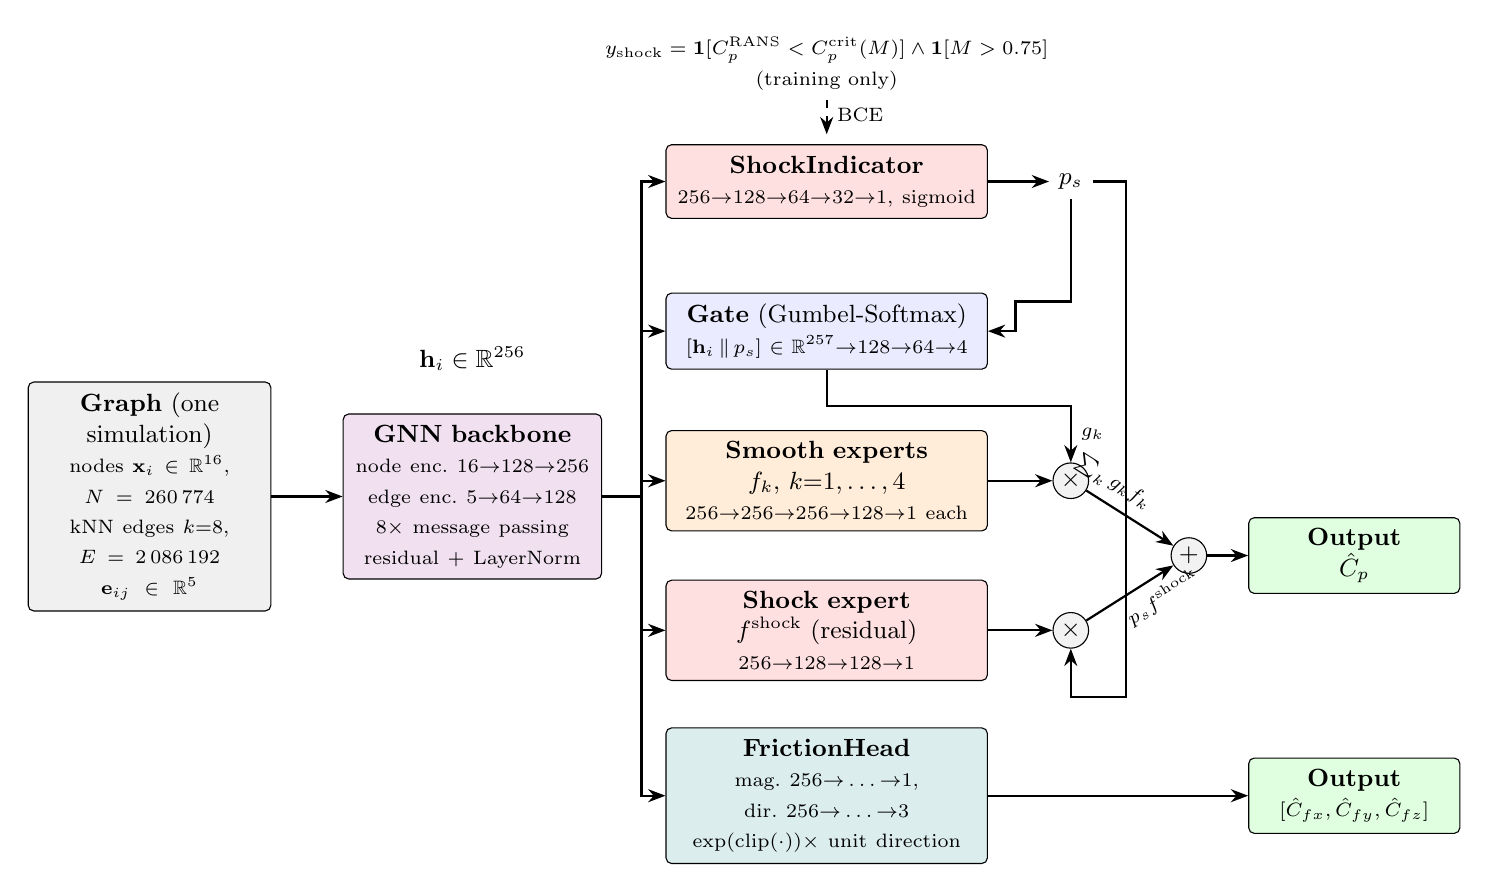
\begin{tikzpicture}[
  font=\small,
  blk/.style={draw, rounded corners=2pt, align=center,
              inner sep=4pt, text width=38mm},
  op/.style={draw, circle, inner sep=1.2pt, fill=gray!10},
  arrow/.style={-{Stealth[length=2.2mm]}, thick}
]
% ---- Input: a graph, not a point ----
\node[blk, fill=gray!12, text width=28mm] (input) at (0,0)
  {\textbf{Graph} (one simulation)\\
  {\scriptsize nodes $\mathbf{x}_i\in\mathbb{R}^{16}$, $N=260\,774$}\\
  {\scriptsize kNN edges $k{=}8$, $E=2\,086\,192$}\\
  {\scriptsize $\mathbf{e}_{ij}\in\mathbb{R}^{5}$}};

% ---- Backbone ----
\node[blk, fill=violet!12, text width=30mm] (bb) at (4.1,0)
  {\textbf{GNN backbone}\\
  {\scriptsize node enc.\ $16{\to}128{\to}256$}\\
  {\scriptsize edge enc.\ $5{\to}64{\to}128$}\\
  {\scriptsize $8\times$ message passing}\\
  {\scriptsize residual $+$ LayerNorm}};
\node (hlab) at (4.1,1.75) {$\mathbf{h}_i\in\mathbb{R}^{256}$};

% ---- Heads ----
\node[blk, fill=red!12] (si) at (8.6,4.0)
  {\textbf{ShockIndicator}\\
  {\scriptsize $256{\to}128{\to}64{\to}32{\to}1$, sigmoid}};
\node[blk, fill=blue!8] (gate) at (8.6,2.1)
  {\textbf{Gate} (Gumbel-Softmax)\\
  {\scriptsize $[\mathbf{h}_i\,\|\,p_s]\in\mathbb{R}^{257}{\to}128{\to}64{\to}4$}};
\node[blk, fill=orange!15] (e1) at (8.6,0.2)
  {\textbf{Smooth experts} $f_k$, $k{=}1,\dots,4$\\
  {\scriptsize $256{\to}256{\to}256{\to}128{\to}1$ each}};
\node[blk, fill=red!12] (se) at (8.6,-1.7)
  {\textbf{Shock expert} $f^{\mathrm{shock}}$ (residual)\\
  {\scriptsize $256{\to}128{\to}128{\to}1$}};
\node[blk, fill=teal!14] (fh) at (8.6,-3.8)
  {\textbf{FrictionHead}\\
  {\scriptsize mag.\ $256{\to}\dots{\to}1$, dir.\ $256{\to}\dots{\to}3$}\\
  {\scriptsize $\exp(\mathrm{clip}(\cdot))\times$ unit direction}};

% ---- Training-only supervision (dashed) ----
\node[align=center] (ysh) at (8.6,5.5)
  {\scriptsize $y_{\mathrm{shock}}=\mathbf{1}[C_p^{\mathrm{RANS}}<C_p^{\mathrm{crit}}(M)]
   \wedge \mathbf{1}[M>0.75]$\\
  {\scriptsize (training only)}};
\draw[-{Stealth[length=2.2mm]}, thick, dashed] (ysh)
  -- node[right, pos=0.45]{\scriptsize BCE} (8.6,4.6);

% ---- Operators and outputs ----
\node (ps) at (11.7,4.0) {$p_s$};
\node[op] (mult)  at (11.7,0.2)  {$\times$};
\node[op] (mult2) at (11.7,-1.7) {$\times$};
\node[op] (plus)  at (13.2,-0.75) {$+$};
\node[blk, fill=green!12, text width=24mm] (outcp) at (15.3,-0.75)
  {\textbf{Output}\\ $\hat{C}_p$};
\node[blk, fill=green!12, text width=24mm] (outcf) at (15.3,-3.8)
  {\textbf{Output}\\
  {\scriptsize $[\hat{C}_{fx},\hat{C}_{fy},\hat{C}_{fz}]$}};

% ---- Wiring ----
\draw[arrow] (input) -- (bb);
\draw[arrow] (bb.east) -- ++(0.5,0) |- (si.west);
\draw[arrow] (bb.east) -- ++(0.5,0) |- (gate.west);
\draw[arrow] (bb.east) -- ++(0.5,0) |- (e1.west);
\draw[arrow] (bb.east) -- ++(0.5,0) |- (se.west);
\draw[arrow] (bb.east) -- ++(0.5,0) |- (fh.west);

% Shock probability paths
\draw[arrow] (si.east) -- (ps);
\draw[arrow] (ps.south) -- ++(0,-1.3) -| ($(gate.east)+(0.35,0)$)
  -- (gate.east);
\draw[arrow] (ps.east) -- (12.4,4.0) -- (12.4,-2.55) -- (11.7,-2.55)
  -- (mult2.south);

% Gate weights
\draw[arrow] (gate.south) -- (8.6,1.15) -- (11.7,1.15)
  -- node[right, pos=0.5]{\scriptsize $g_k$} (mult.north);

% Expert paths
\draw[arrow] (e1.east) -- (mult.west);
\draw[arrow] (se.east) -- (mult2.west);

% Combination
\draw[arrow] (mult) -- node[sloped, above, pos=0.18]{\scriptsize $\textstyle\sum_k g_k f_k$} (plus);
\draw[arrow] (mult2) -- node[sloped, below, pos=0.75]{\scriptsize $p_s f^{\mathrm{shock}}$} (plus);
\draw[arrow] (plus) -- (outcp);
\draw[arrow] (fh.east) -- (outcf);
\end{tikzpicture}}
\caption{AeroSurrogate architecture and data flow (4\,603\,918
  parameters): GNN backbone, ShockIndicator, shock-gated $C_p$ mixture
  of experts, and friction head.  Dashed elements exist only at
  training time (BCE supervision).}
\label{fig:architecture}
\end{figure}

\subsection{Spatial backbone}
\label{sec:backbone}

The graph is built once per simulation: its $N = 260\,774$ nodes are
the surface mesh points carrying the sixteen features of
Section~\ref{sec:dataset}, its edges the $k=8$ nearest neighbours of
the node coordinates, $E = 8N = 2\,086\,192$ directed edges from a
KD-tree, so no mesh connectivity is required and a bare point cloud
suffices.  Each edge carries $\mathbf{e}_{ij} = (\delta x, \delta y,
\delta z, \|\boldsymbol{\delta}\|,
\mathbf{n}_i\!\cdot\!\mathbf{n}_j)$.  A node encoder
$16\!\to\!128\!\to\!256$ lifts $\mathbf{x}_i$ to
$\mathbf{h}_i\in\mathbb{R}^{256}$ and an edge encoder
$5\!\to\!64\!\to\!128$ lifts $\mathbf{e}_{ij}$; each of the eight
message-passing layers then applies a residual update normalised by
LayerNorm~\cite{Ba2016}, messages being aggregated at the destination
by concatenated mean and maximum:
\begin{equation}
  \mathbf{m}_{i\to j} =
    \phi_{m}\bigl([\mathbf{h}_i \,\|\, \mathbf{e}_{ij}]\bigr),
  \qquad
  \mathbf{h}_j \leftarrow
    \mathrm{LN}\Bigl(\mathbf{h}_j + \phi_{u}\bigl([\mathbf{h}_j \,\|\,
      \mathrm{mean}\,\mathbf{m} \,\|\, \mathrm{max}\,\mathbf{m}]\bigr)\Bigr)
  \label{eq:backbone}
\end{equation}
with $\phi_m: 384\!\to\!256\!\to\!256$ and
$\phi_u: 768\!\to\!256\!\to\!256$.  Eight layers give an eight-hop
receptive field, so each latent summarises a patch of surface rather
than a point.  All hidden layers use LayerNorm, SiLU~\cite{Elfwing2018}
and dropout 0.1, the gate excepted.

\subsection{ShockIndicator and shock-gated experts}
\label{sec:moe}

The ShockIndicator is an MLP $256\!\to\!128\!\to\!64\!\to\!32\!\to\!1$
with a sigmoid output $p_{s,i}\in[0,1]$, supervised by
$y_{\mathrm{shock}}$, Eq.~(\ref{eq:labels}), through the cross-entropy
term of Eq.~(\ref{eq:loss}).  Reading the backbone latent rather than
the raw point features makes it \emph{spatial}: it conditions on the
pressure-gradient structure that defines a shock, and since the label
is a conjunction it detects the transonic shock regime rather than
local supersonic flow.  On eight held-out test simulations it attains
precision $0.8964$, recall $0.9927$ and $F_1 = 0.9421$.

The ShockGatedMoE predicts the pressure coefficient alone.  Its gate
maps $[\mathbf{h}_i\,\|\,p_{s,i}]\in\mathbb{R}^{257}$ through
$257\!\to\!128\!\to\!64\!\to\!4$ to $K=4$ routing logits
$\mathbf{l}_i$; each smooth expert is an MLP
$256\!\to\!256\!\to\!256\!\to\!128\!\to\!1$ and the shock expert a
smaller $256\!\to\!128\!\to\!128\!\to\!1$ entering as an additive
residual scaled by $p_s$:
\begin{equation}
  \hat{C}_{p,i} =
    \sum_{k=1}^{K} g_{k}(\mathbf{h}_i, p_{s,i})\, f_{k}(\mathbf{h}_i)
    \;+\; p_{s,i}\, f^{\mathrm{shock}}(\mathbf{h}_i)
  \label{eq:forward_cp}
\end{equation}
The residual splits the loading into a smooth background and a shock
perturbation whose sharpness is inherited from the sigmoid of the
indicator: it vanishes where $p_s\!\approx\!0$ and supplies the learned
pressure jump inside the supersonic pocket, as in sensor-activated
shock capturing~\cite{Discacciati2020}, except that here both sensor
and correction are learned.  Because the gate is per node its
specialisation is spatial rather than per condition: the mean weight
of expert $E_0$ rises from $0.1451$ off shock to $0.4722$ on labelled
shock nodes, emerging from routing rather than from explicit
labels~\cite{Jacobs1991,Shazeer2017}.  In training the gate uses the
Gumbel-Softmax relaxation~\cite{Jang2017},
$\mathbf{g}_i = \mathrm{softmax}\bigl((\mathbf{l}_i+\mathbf{G}_i)/
\tau\bigr)$ with $G_k = -\log(-\log u_k)$ and $\tau$ annealed from
$1.0$ to $0.3$ over 200 epochs; at inference it is a deterministic
softmax, close to one-hot at a mean per-node entropy of $0.080$
against $\log K = 1.3863$.

\subsection{Friction head}
\label{sec:friction}

The friction vector is predicted by a head reading $\mathbf{h}_i$ in
parallel with the $C_p$ branch and factorised into a magnitude and a
unit direction, since $\|\mathbf{C}_f\|$ spans orders of magnitude
over the surface: branches $256\!\to\!256\!\to\!256\!\to\!128\!\to\!1$
and $256\!\to\!256\!\to\!256\!\to\!128\!\to\!3$ give a log-magnitude,
clipped and exponentiated, and an $L_2$-normalised direction,
\begin{equation}
  \hat{\mathbf{C}}_{f,i} =
    \exp\!\bigl(\mathrm{clip}(f_{\mathrm{mag}}(\mathbf{h}_i),\,-10,\,5)\bigr)\;
    \frac{f_{\mathrm{dir}}(\mathbf{h}_i)}{\|f_{\mathrm{dir}}(\mathbf{h}_i)\|}
  \label{eq:forward_cf}
\end{equation}
The head is not gated by $p_s$, so the discontinuity mechanism acts on
the pressure alone.

\subsection{Loss function and training}
\label{sec:loss}\label{sec:training}

Training minimises a four-term objective over the $N$ nodes of one
simulation graph:
\begin{equation}
  \begin{split}
    \mathcal{L} ={}&
      w_f\underbrace{\frac{1}{N}\sum_{i=1}^{N} w_i\,
        \bigl(\hat{C}_{p,i} - C_{p,i}\bigr)^{2}}_{\text{shock-weighted }C_p\text{ MSE}}
      \;+\; \lambda_{s}\,
      \underbrace{\mathrm{BCE}\bigl(\mathrm{shock\_logit},\,
        y_{\mathrm{shock}}\bigr)}_{\text{indicator supervision}} \\[2ex]
    &\;-\; \lambda_{\mathrm{lb}}\,
      \underbrace{H(\bar{\mathbf{g}})}_{\text{load balance}}
      \;+\; \lambda_{\mathrm{fric}}\,w_f\,
      \underbrace{\mathcal{L}_{\mathrm{fric}}}_{\text{friction}}
  \end{split}
  \label{eq:loss}
\end{equation}
with load balance
$H(\bar{\mathbf{g}}) = -\sum_{k}\bar{g}_k\log\bar{g}_k$,
$\bar{g}_k = N^{-1}\sum_i g_{i,k}$, and friction term
\begin{equation}
  \mathcal{L}_{\mathrm{fric}} =
    \frac{1}{N}\sum_{i=1}^{N}
      \bigl(\log\|\hat{\mathbf{C}}_{f,i}\| -
            \log\|\mathbf{C}_{f,i}\|\bigr)^{2}
    \;+\;
    \frac{1}{N}\sum_{i=1}^{N}
      \min\!\left(\frac{\|\mathbf{C}_{f,i}\|}
                       {\overline{\|\mathbf{C}_{f}\|}},\,5\right)
      \bigl(1-\cos(\hat{\mathbf{C}}_{f,i},\mathbf{C}_{f,i})\bigr)
  \label{eq:fric}
\end{equation}
Here $w_i = 1 + \lambda_{\mathrm{sw}}\,y_{\mathrm{shock},i}$,
$\lambda_{s}=0.1$, $\lambda_{\mathrm{lb}}=0.01$,
$\lambda_{\mathrm{sw}}=5.0$ and $\lambda_{\mathrm{fric}}=3.0$, so
shock nodes carry $6\times$ weight in the $C_p$ term and none in the
friction one; $w_f\in\{1.0,\,0.5\}$ is the ONERA regression-challenge
confidence weight shipped with the database, which scales the two
regression terms alone and makes the weighted $R^{2}$ of
Section~\ref{sec:results} comparable with the reference results.  The
load-balance entropy is \emph{maximised}, that is, subtracted from the
minimised objective: it vanishes when the gate collapses onto a single
expert, so adding it instead drives the very collapse it is meant to
prevent (Section~\ref{sec:results}); here it settles at $1.3827$,
$99.7\%$ of uniform.

Training runs in two stages, \emph{stage~A} end-to-end from scratch
and \emph{stage~B} a head-only fine-tune resuming from that checkpoint
with the backbone frozen, which is the reported model.  Optimisation
uses AdamW, peak learning rate $10^{-3}$ after three warmup epochs
cosine-annealed to $10^{-6}$, weight decay $10^{-5}$, gradient-norm
clipping at 1.0, and up to 200 epochs per stage with patience 8;
activation checkpointing makes one simulation graph a single optimiser
step.  Checkpoints are
selected on the \emph{unweighted} $R^{2}(C_p)$ over the 16 validation
simulations drawn from the \emph{test} split; the point-wise baseline
is quoted from its own protocol, a $10\%$ random sample of all 156
test simulations, 4\,068\,074 points, so its column of
Table~\ref{tab:results} is not measured on the same population.

At inference no solver output is required: the model consumes the
surface nodes and the flight condition, from which every feature
follows analytically, and returns the four coefficients in one forward
pass with $p_{s,i}$ as an interpretable by-product.  It consumes the
surface \emph{as a whole}, however, and so cannot score an isolated
point, a deployment regression relative to the point-wise
formulation.

% ================================================================
\section{RESULTS AND DISCUSSION}
\label{sec:results}
% ================================================================

\subsection{Aerodynamic coefficient prediction}

Table~\ref{tab:results} reports the coefficient-of-determination
scores over the 140 held-out simulations and 36\,508\,360 surface
points.  In physical units the mean absolute error on $C_p$ is
$0.0276$ globally and $0.0405$ on the shock subset, and the
confidence-weighted $R^{2}$ in which form the reference results for
this database are reported is $0.9768$ for $C_p$.  In the table,
\emph{nearest cond.} is the no-learning baseline described below,
\emph{collapsed gate} is the run trained before the load-balancing
sign correction, \emph{from scratch} is joint end-to-end training with
the corrected loss, and \emph{two-stage} is the reported model:
end-to-end pre-training then a head-only fine-tune with the backbone
frozen.

\begin{table}[htbp]
\centering
\caption{Coefficient of determination on the held-out test set: 140
  simulations (36\,508\,360 surface points) disjoint from both
  training and model selection.  Columns are defined in the text; the
  two-stage column is the reported model and the point-wise one is
  measured on a different protocol.}
\label{tab:results}
\setlength{\tabcolsep}{4pt}
\begin{tabular}{llccccc}
\toprule
\textbf{Subset} & \textbf{Coef.} & \textbf{nearest cond.}
  & \textbf{point-wise} & \textbf{collapsed gate}
  & \textbf{from scratch} & \textbf{two-stage} \\
\midrule
global    & $R^{2}(C_p)$    & 0.9159 & 0.9506 & 0.9549 & 0.9580 & \textbf{0.9729} \\
          & $R^{2}(C_{fx})$ & 0.8729 & 0.8512 & 0.8665 & 0.8775 & \textbf{0.9172} \\
          & $R^{2}(C_{fy})$ & 0.8823 & 0.8463 & 0.8443 & 0.8509 & \textbf{0.9027} \\
          & $R^{2}(C_{fz})$ & 0.8629 & 0.8555 & 0.8796 & 0.8806 & \textbf{0.9209} \\
\midrule
shock     & $R^{2}(C_p)$    & 0.7779 & 0.8827 & 0.8814 & 0.8956 & \textbf{0.9350} \\
          & $R^{2}(C_{fx})$ & 0.8524 & 0.8390 & 0.8231 & 0.8445 & \textbf{0.8923} \\
          & $R^{2}(C_{fy})$ & 0.8843 & 0.8292 & 0.7867 & 0.8063 & \textbf{0.8692} \\
          & $R^{2}(C_{fz})$ & 0.9047 & 0.8643 & 0.8592 & 0.8677 & \textbf{0.9076} \\
\midrule
transonic & $R^{2}(C_p)$    & 0.9600 & 0.9629 & 0.9669 & 0.9698 & \textbf{0.9842} \\
subsonic  & $R^{2}(C_p)$    & 0.8078 & 0.9236 & 0.9259 & 0.9303 & \textbf{0.9471} \\
\bottomrule
\end{tabular}
\end{table}

The nearest-training-condition baseline performs no learning at all:
for each held-out simulation it copies the surface field of the
training condition closest to it in the normalised
$(M_{\infty}, \alpha, \Pi)$ space.  The median normalised distance to
that neighbour is $0.0333$ and the maximum $0.1000$, so the sampling
is dense enough for the baseline to be demanding rather than a straw
man; it reaches $R^{2}(C_p) = 0.9159$ globally, which places most of
the aggregate score within reach of interpolation between neighbouring
conditions.  Where it fails is where the architecture is aimed:
$0.7779$ on the shock subset against $0.9350$, and $0.8078$ on the
subsonic subset against $0.9471$.  A neighbouring condition puts the
shock almost in the right position, and is penalised on both sides of
the offset.

The gap between pressure and friction accuracy is structural: surface
pressure is set by the outer, essentially inviscid flow and is a
largely local function of the input vector, whereas skin friction is a
wall-gradient quantity, two to three orders smaller, encoding the
upstream history of the boundary layer, non-local information that
eight rounds of message passing over an isotropic $k{=}8$ graph
propagate only in part.  Every regressor evaluated on this database
shows the same ordering~\cite{Peter2025}.

The three trained columns of Table~\ref{tab:results} separate two
independent corrections, and they are not the same size.  The
load-balance term was an entropy that had been added to, rather than
subtracted from, the minimised objective, and it therefore drove the
gate toward the collapse it was meant to prevent; repairing its sign,
with the training schedule held fixed, moves global $R^{2}(C_p)$ from
$0.9549$ to $0.9580$ and the shock-subset score from $0.8814$ to
$0.8956$.  Adding the two-stage schedule on top of the corrected loss
is worth substantially more, $0.9580$ to $0.9729$ globally and
$0.8956$ to $0.9350$ on shock nodes, about $2.8\times$ the sign
correction inside the shock region.  The collapsed-gate run reaches
only $0.8814$ on shock $C_p$, no better than the $0.8827$ of the
point-wise predecessor on its own sample: the mixture pays for itself
only once the gate is balanced.

Suppressing the additive shock residual $p_s\,f^{\mathrm{shock}}(\mathbf{h}_i)$
at inference, with every weight otherwise unchanged, raises the $C_p$ mean
absolute error on the shock nodes of eight held-out test simulations from
$0.0458$ to $0.1370$: the residual removes $66.6\%$ of the error the smooth
mixture alone would incur there, and on those same nodes it carries $43.4\%$
of the magnitude of the smooth output.  That is the discontinuity mechanism
measured directly rather than inferred from the aggregate scores.  The schedule
comparison, by contrast, rests on a single run per arm, matched in data,
loss and setup and both stopped on patience, so it cannot separate a
curriculum effect from a fortunate initialisation.

The model scores better in the transonic regime than in the subsonic
one ($R^{2}(C_p) = 0.9842$ against $0.9471$), which follows from the
objective: the shock label requires $M_{\infty} > 0.75$, so the
six-fold weight $w_i$ can never reach a subsonic node, and just over a
quarter of the held-out transonic points carry the label
(6\,830\,670 of 26\,077\,400).

\subsection{How far the shock criterion compresses}
\label{sec:symbolic}

Because the indicator is supervised on a physical label, it is fair to
ask whether it can be written down.  For the point-wise predecessor of
this model, whose indicator read the nine interpretable node variables
directly, symbolic regression recovers the five-node expression
$p_s = \tanh(\exp(C_p^{\mathrm{crit}}(M)/\eta))$, $\eta$ the normalised
span station, which activates with Mach and towards the tip.
Substituting it there costs $0.0085$ in $R^{2}(C_p)$ but $0.1005$ in
$R^{2}(C_{fy})$: the pressure criterion survives compression, the
lateral friction does not.

Against the spatial indicator the same search does not close.  It
recovers the same $\exp(C_p^{\mathrm{crit}}/\sqrt{\eta})$ core, which
corroborates the earlier expression independently, yet a $29$-node
expression reaches only $R^{2}=0.4095$ against the indicator's own
output where an unconstrained regressor on the identical variables
reaches $0.8850$.  The information is local; the closed form is what
cannot hold it.  Once the indicator sees an eight-hop neighbourhood
its criterion stops being compactly expressible, which is the same
richness that lifts the shock-subset score.

\subsection{Full-aircraft surface fields}

Figures~\ref{fig:fields_cp} and \ref{fig:fields_cf} compare the RANS
reference, the AeroSurrogate prediction and the signed error
(CFD $-$ model) for $C_p$ and for the skin-friction magnitude
$\lvert\mathbf{C}_f\rvert$, over both aircraft surfaces, for six
held-out flight conditions spanning the envelope from $M{=}0.30$,
$\alpha{=}-6^{\circ}$ to $M{=}0.90$, $\alpha{=}6^{\circ}$, none of
which took any part in model selection.  All six rows share a single
field scale and a single error scale, so panels may be compared across
conditions; Figure~\ref{fig:fields_sim147} shows the most demanding of
the six on its own.

\begin{figure}[p]
\centering
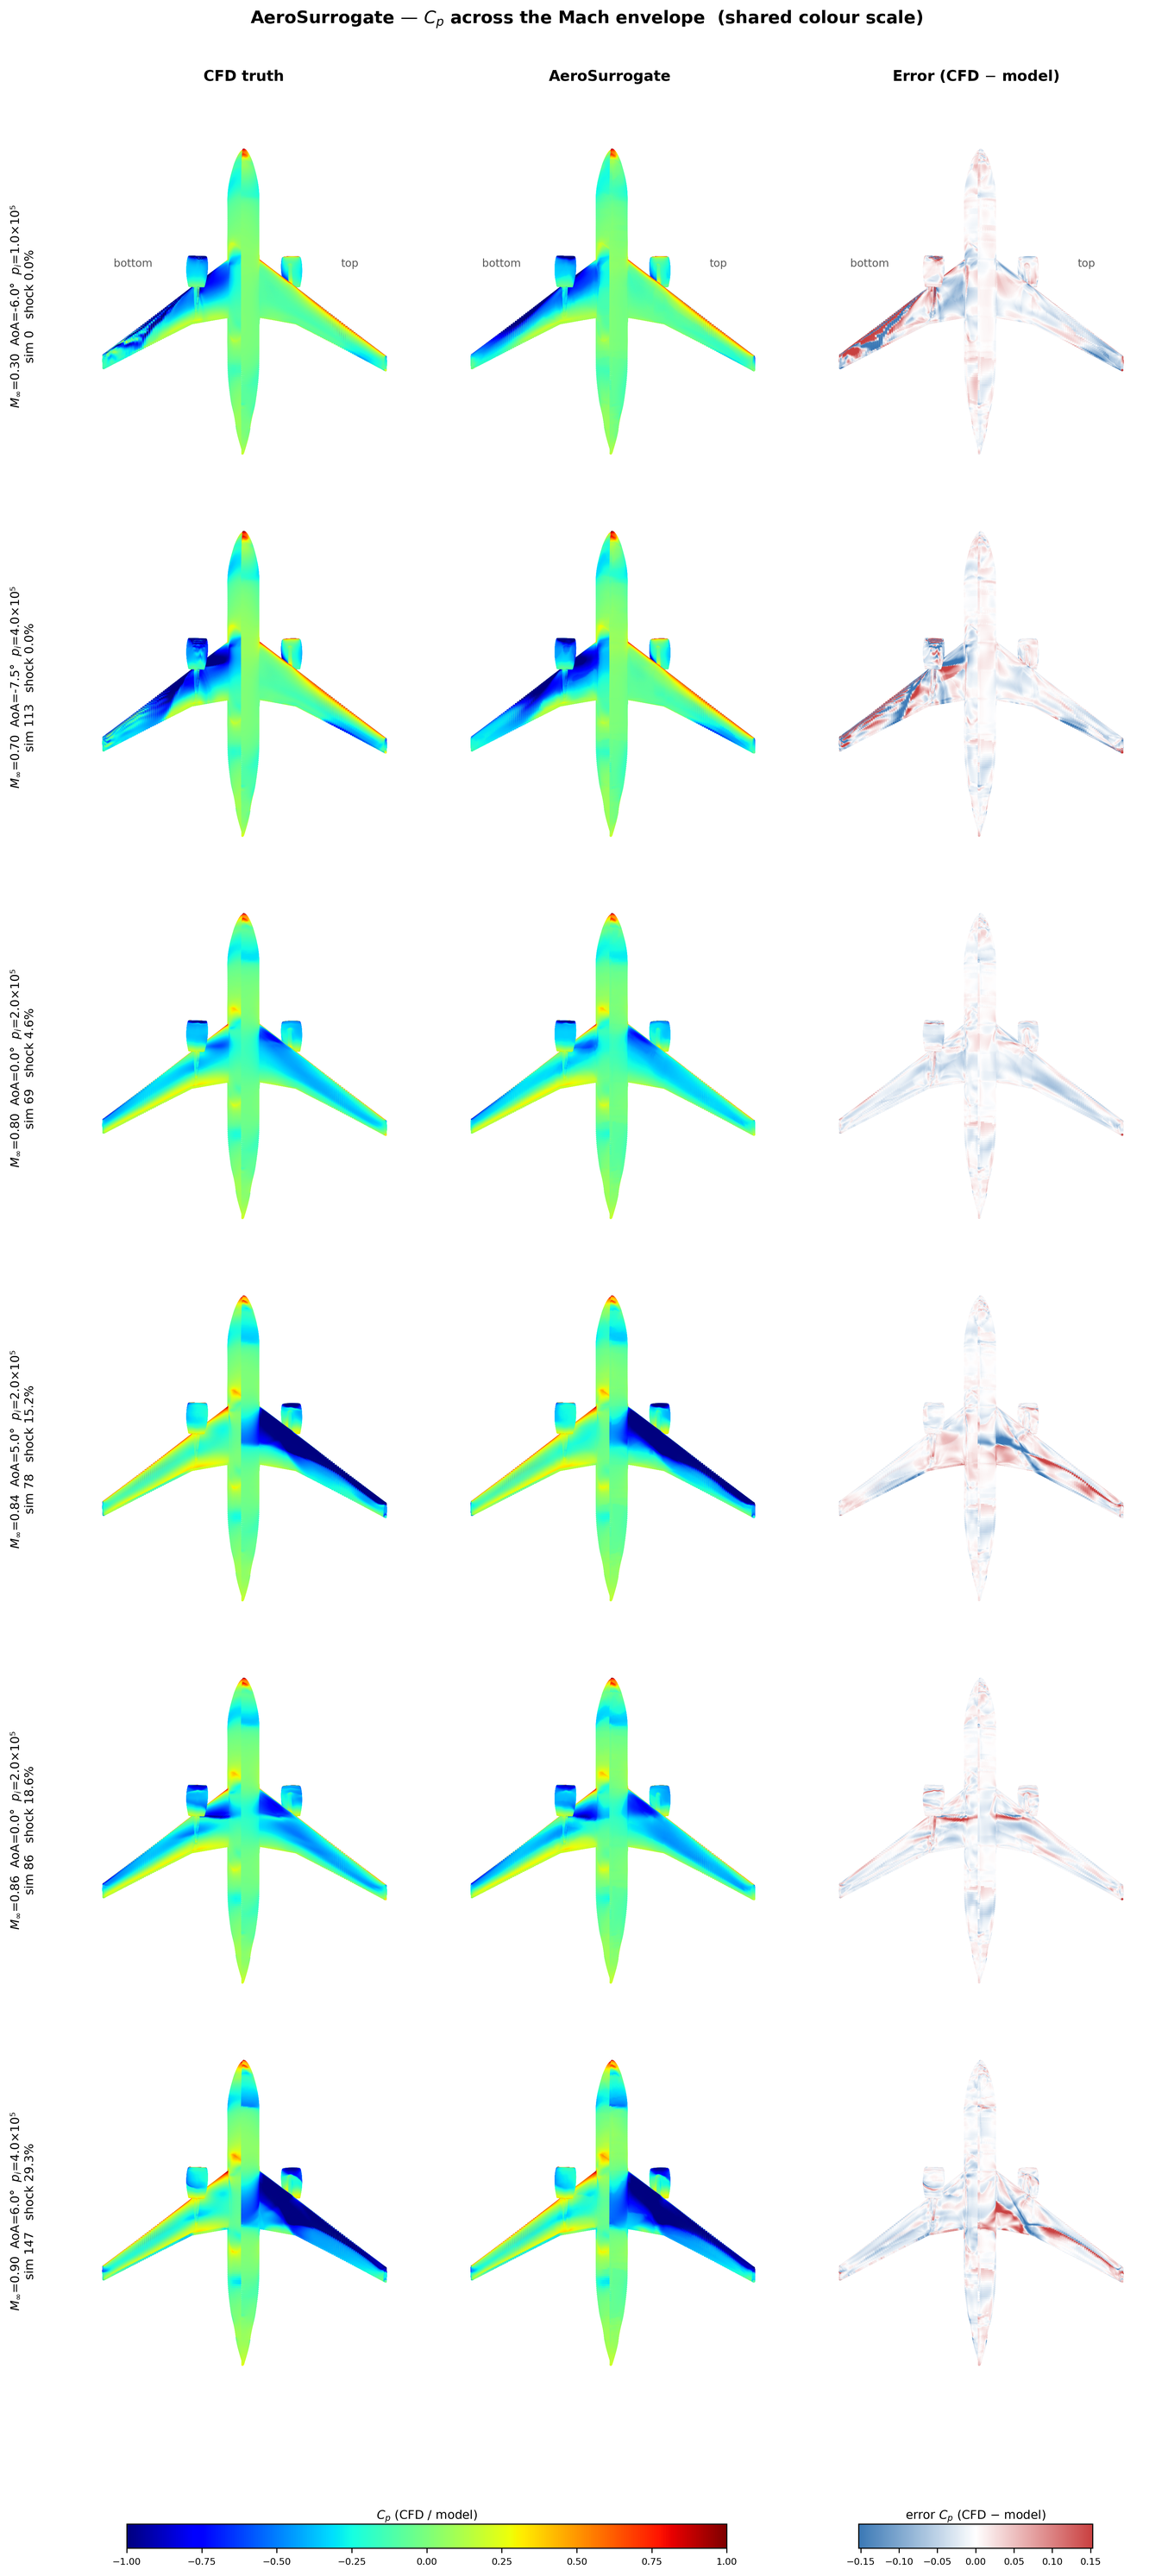
\includegraphics[height=0.86\textheight]{figures/v2_conditions_cp.png}
\caption{Pressure coefficient over six held-out flight conditions, one
  per row: CFD reference (left), AeroSurrogate prediction (centre) and
  signed error, CFD $-$ model (right), on scales shared by all rows.
  Left half-model is the lower surface, right half-model the upper.
  Row labels give $M_{\infty}$, $\alpha$, total pressure $\Pi$
  (printed $p_i$), simulation index and shock-labelled node fraction.}
\label{fig:fields_cp}
\end{figure}

\begin{figure}[p]
\centering
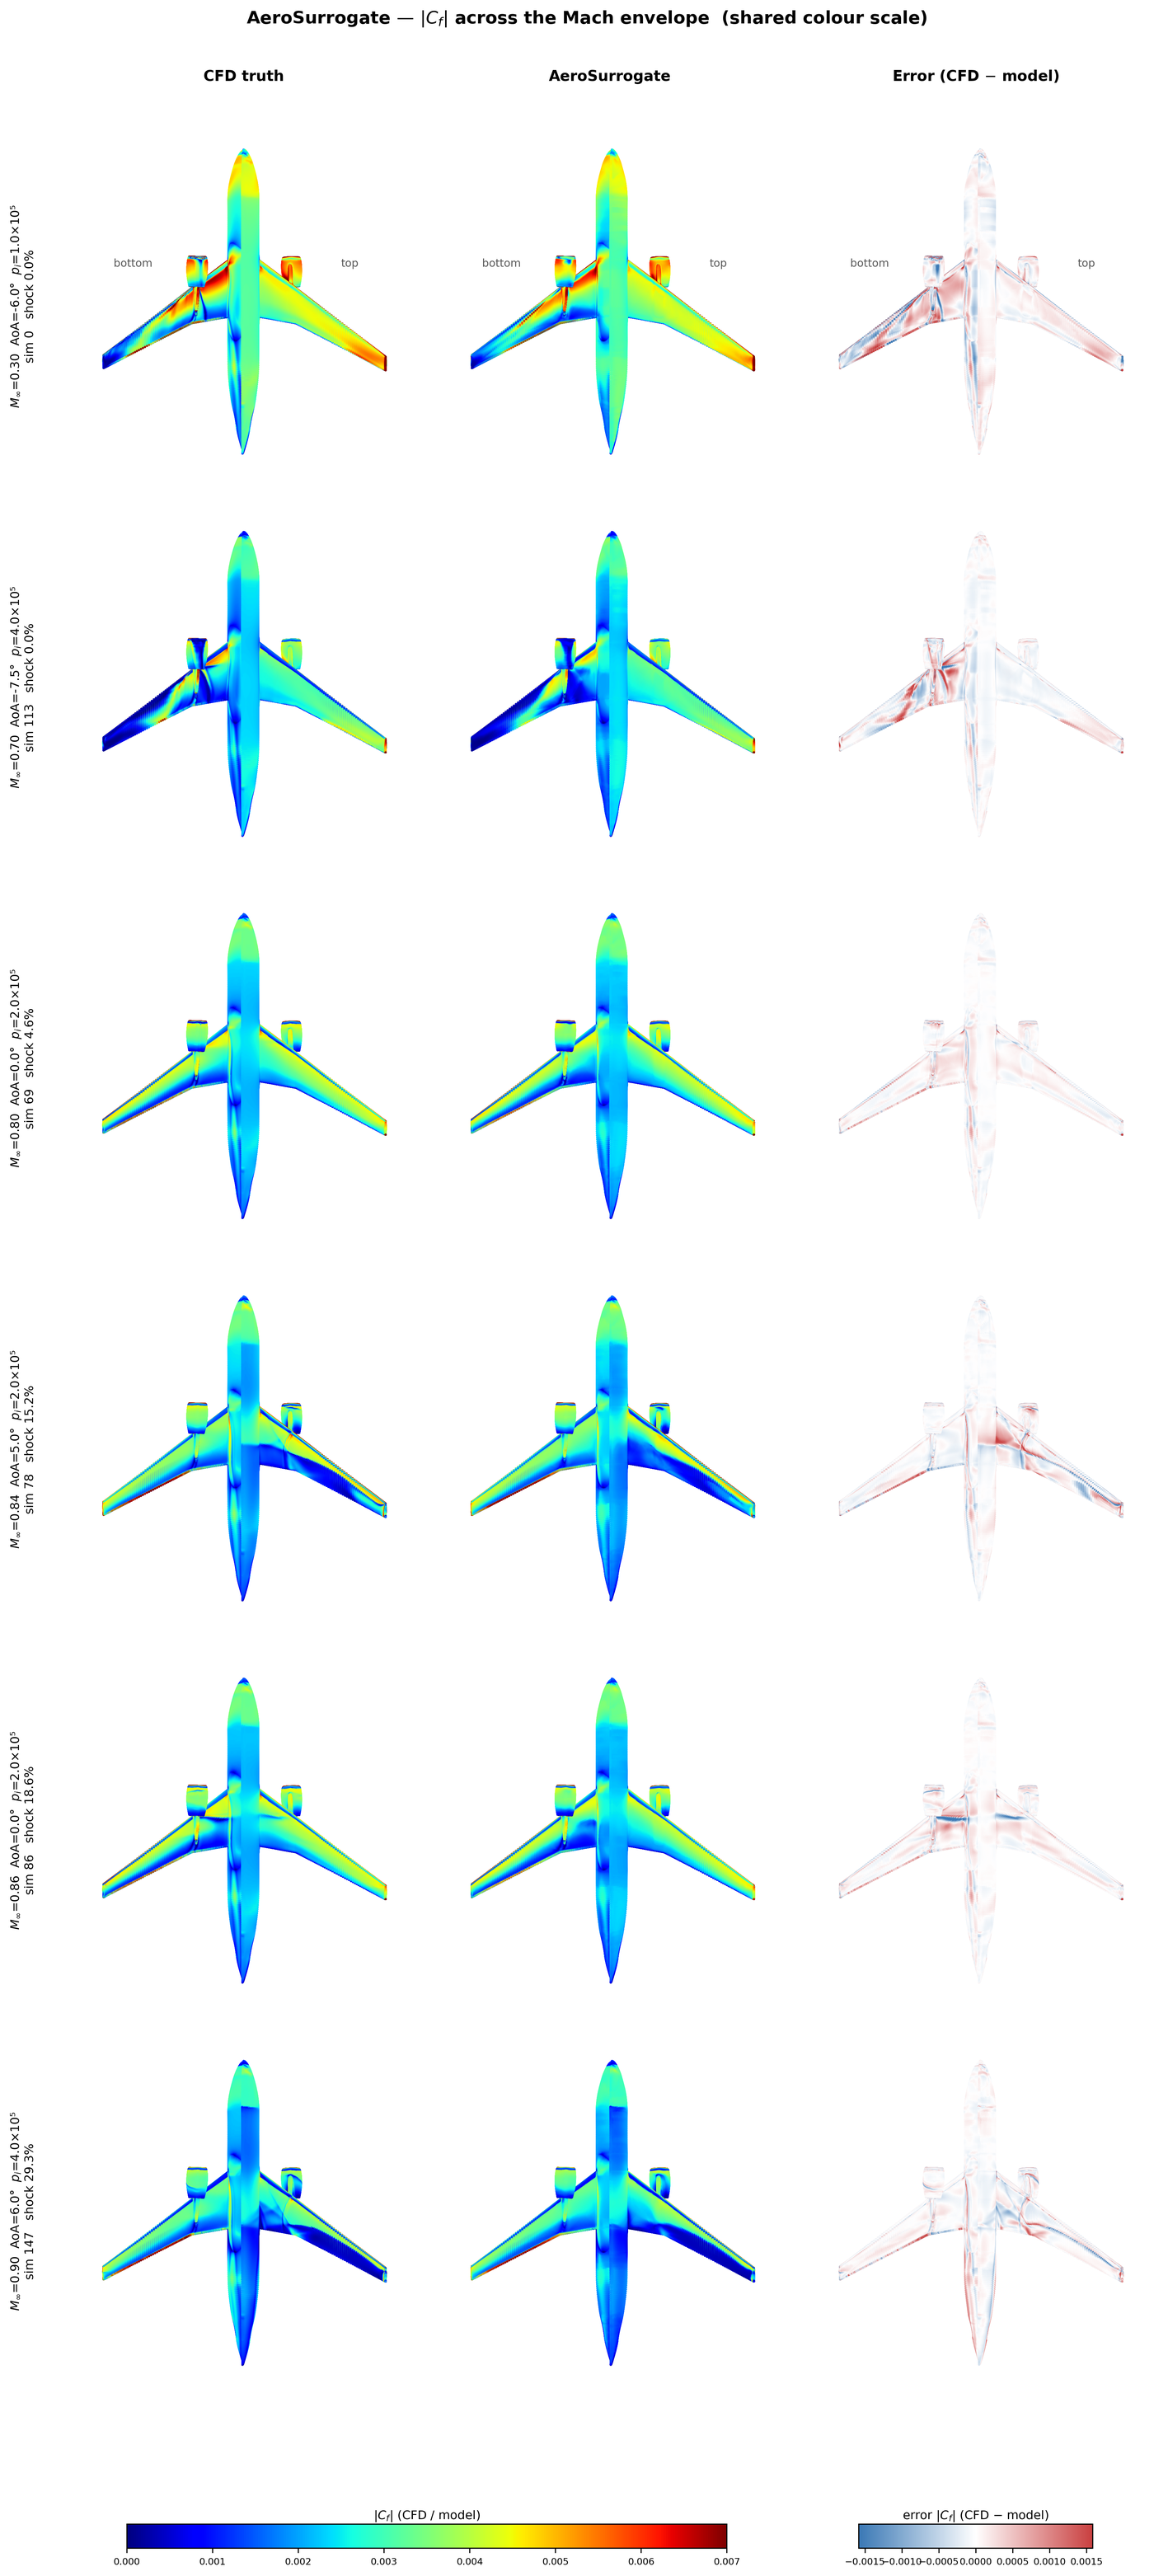
\includegraphics[height=0.90\textheight]{figures/v2_conditions_cf.png}
\caption{Skin-friction magnitude
  $\lvert\mathbf{C}_f\rvert=\lVert(C_{fx},C_{fy},C_{fz})\rVert_{2}$ over
  the same six held-out conditions and in the same layout as
  Figure~\ref{fig:fields_cp}.}
\label{fig:fields_cf}
\end{figure}

The predicted fields reproduce the characteristic structure of each
regime.  The two subsonic rows show the loading redistribution toward
the lower surface induced by the negative incidence, without spurious
oscillations; from the third row onward the upper-wing supersonic
plateau appears at the correct chord-wise and span-wise station and,
as Mach and incidence increase down the figure, strengthens, extends
outboard and moves aft, together with the marked drop of
$\lvert\mathbf{C}_f\rvert$ over the same region in
Figure~\ref{fig:fields_cf}.  The shock-labelled node fraction rises
from $0.0\%$ in the two subsonic rows to $29.3\%$ in the bottom one,
and the surrogate tracks the displacement throughout.

The error maps are signed rather than relative, since an error
normalised by the local coefficient saturates wherever that
coefficient crosses zero.  The error is not largest where the shocks
are: the two visibly worst rows are the two lowest-Mach conditions,
neither of which carries a shock-labelled node.  Within each row it
concentrates at the wing--body junction, the inboard wing and thin
bands along the leading and trailing edges, where the surface field
varies over a length scale comparable to the node spacing and
therefore over few graph hops; over the outer wing, including the
supersonic plateau itself, it is close to zero.

\begin{figure}[htbp]
\centering
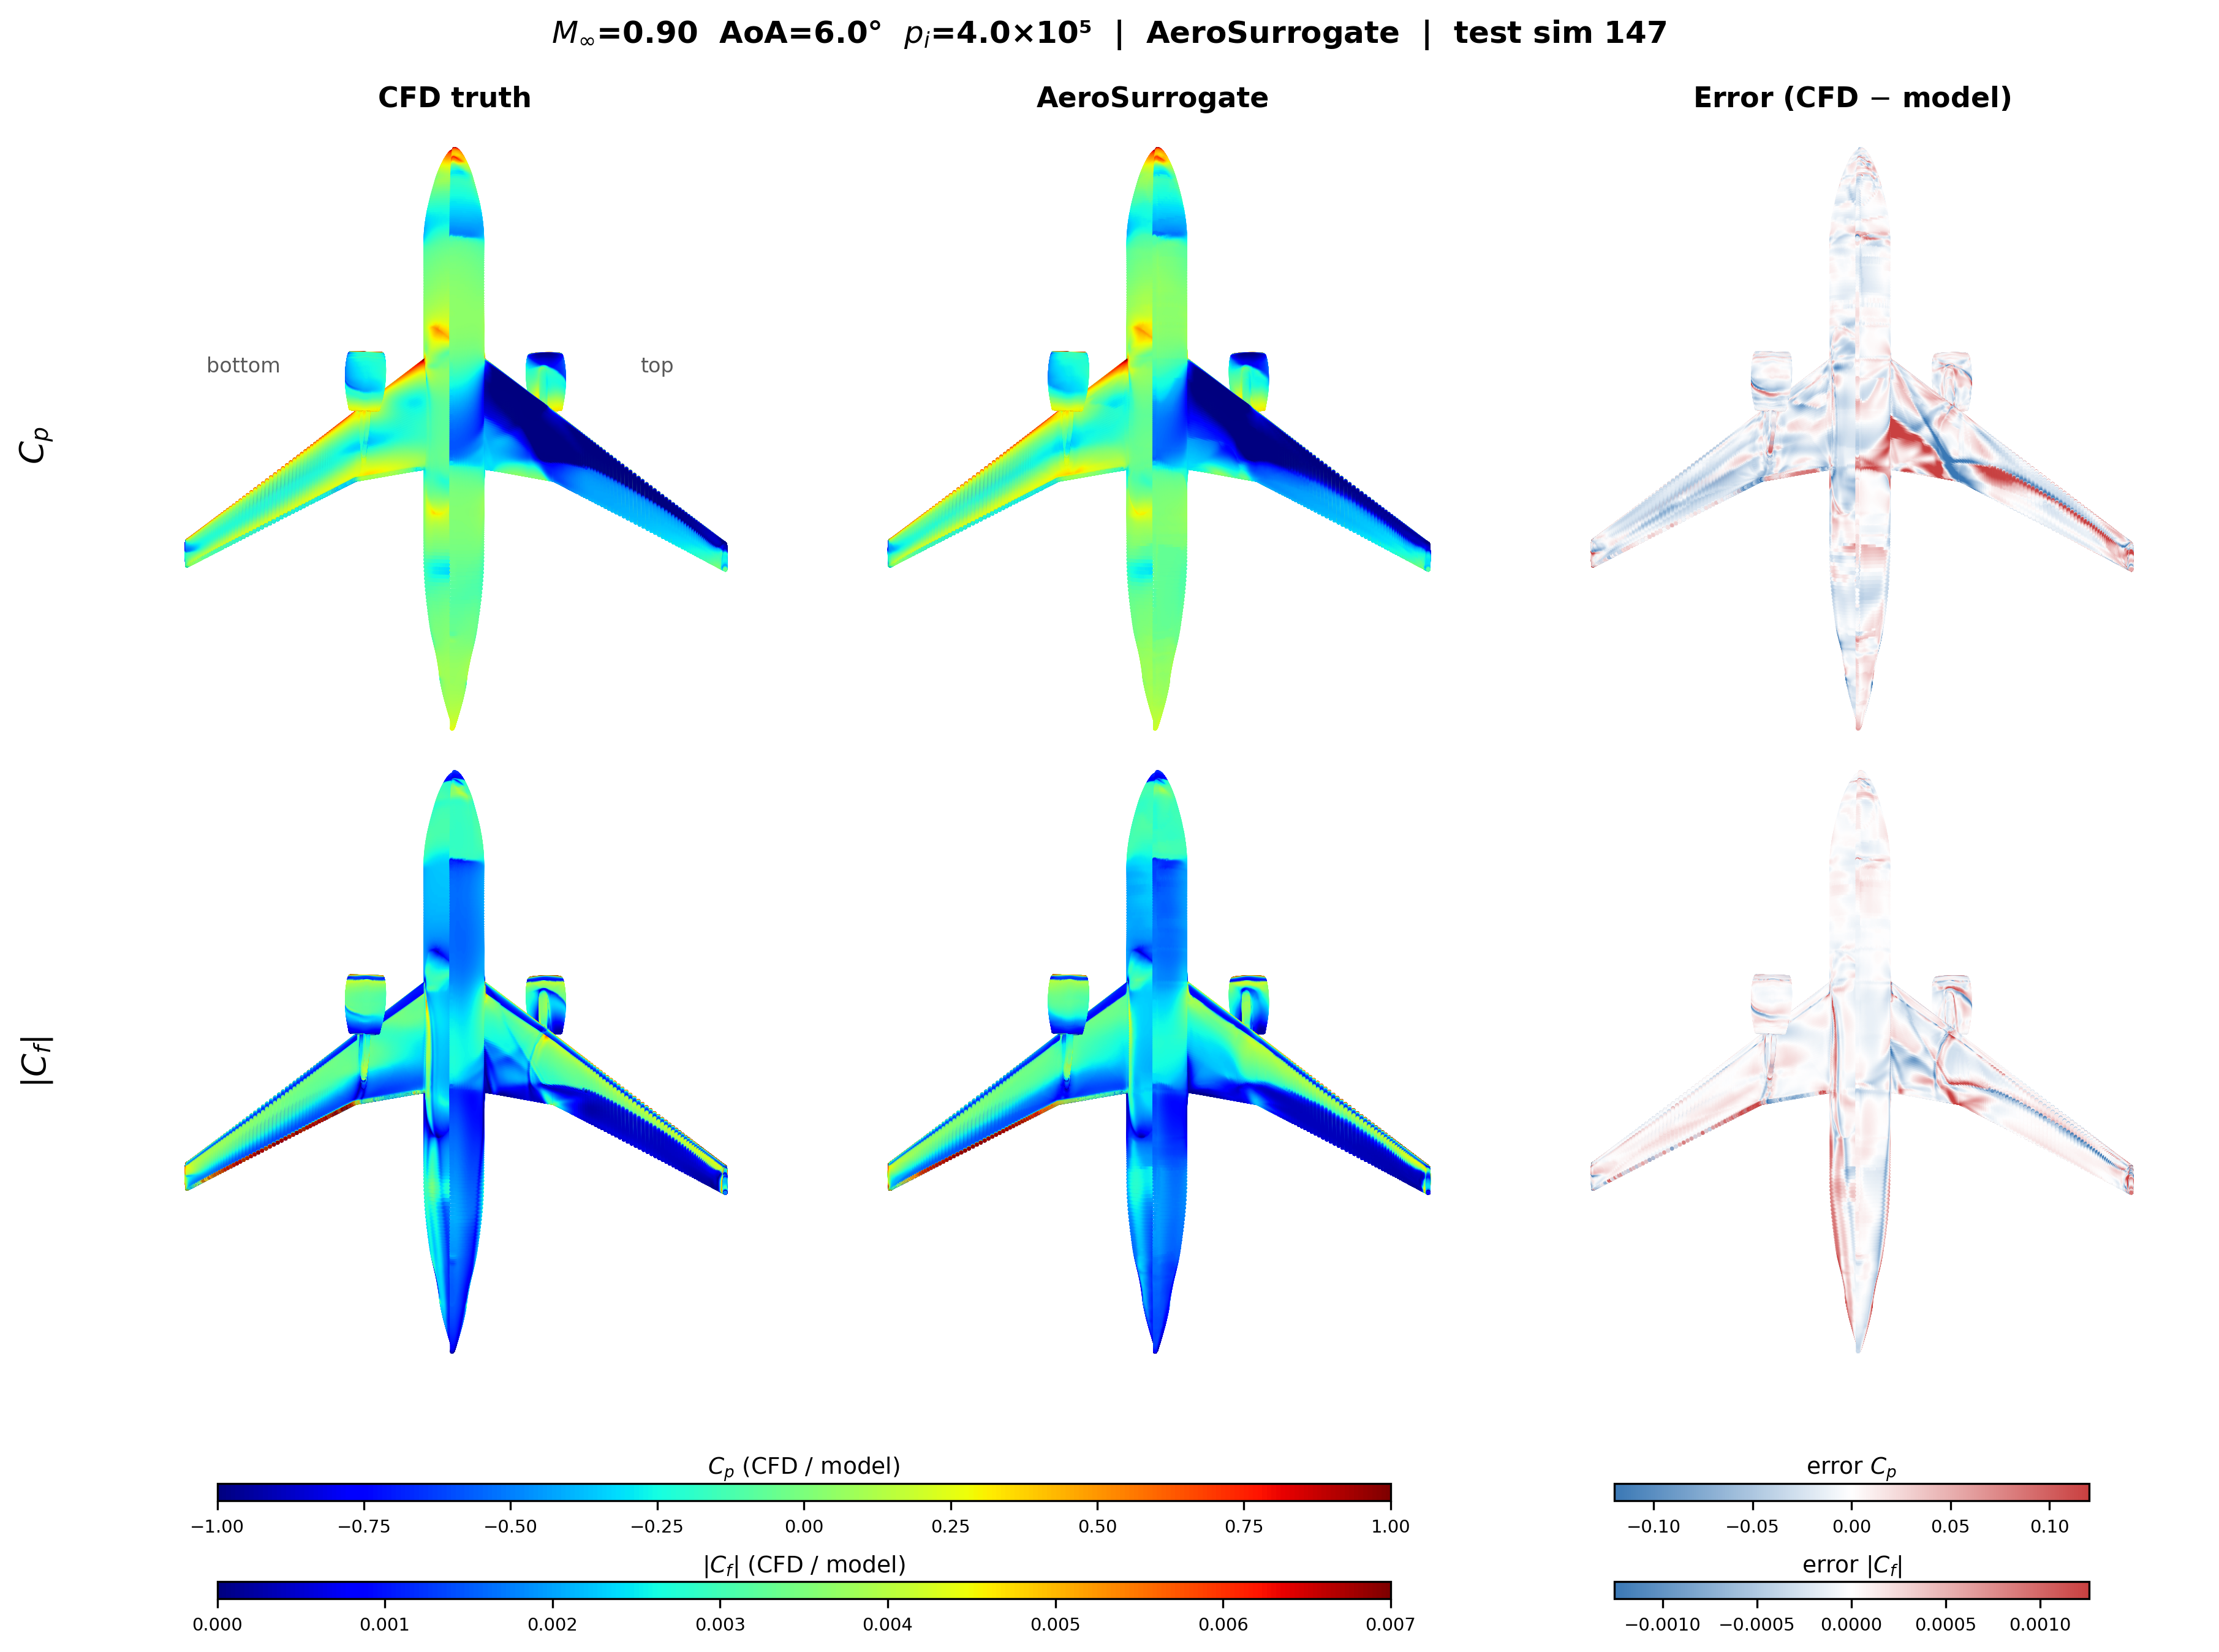
\includegraphics[width=0.78\textwidth]{figures/v2_surface_fields_sim147_wide.png}
\caption{The most demanding condition of the six at full resolution
  ($M_{\infty}{=}0.90$, $\alpha{=}6^{\circ}$, $\Pi{=}4{\times}10^{5}$,
  test simulation 147; $29.3\%$ of its nodes are shock-labelled).
  Each panel places the lower surface left of the upper surface.}
\label{fig:fields_sim147}
\end{figure}


% ================================================================
\section{CONCLUSIONS}
\label{sec:conclusions}
% ================================================================

A physics-aware surrogate for transonic aerodynamic surfaces has been
presented, coupling a spatial graph backbone over the surface mesh to a
shock-gated Mixture of Experts head for $C_p$ and a dedicated friction
head.  On the 140 held-out simulations, 36\,508\,360 surface points, it
reaches $R^{2}(C_p)=0.9729$ globally and $0.9350$ on shock nodes.  That
margin is not an artefact of a densely sampled envelope: a
nearest-training-condition baseline reaches $0.9159$ globally but only
$0.7779$ on shock nodes, so the architecture earns its place where the
physics is hard.  Deleting the shock residual raises the shock-node
$C_p$ mean absolute error from $0.0458$ to $0.1370$; correcting the
load-balancing sign is worth $+0.0142$ on the shock subset, and
maturing the backbone before fine-tuning the head a further $+0.0394$.
Labels read off the RANS pressures keep inference solver-free and are
still recovered with precision $0.8964$ and recall $0.9927$.

Future work will repeat the two-stage and from-scratch arms over several
initialisations, to separate the curriculum effect from seed variance,
and revisit the closed-form criterion of Section~\ref{sec:symbolic} for
the spatial indicator.


% ================================================================
%  ACKNOWLEDGEMENTS
% ================================================================

\section*{ACKNOWLEDGEMENTS}

This work is part of the projects HERFUSE (GA No 101140567), funded by the
European Union, and TIFON (PLEC2023-010251), funded by
MCIN/AEI/\allowbreak 10.13039/\allowbreak 501100011033.

% ================================================================
%  REFERENCES
% ================================================================

\begin{thebibliography}{14}
\setlength{\itemsep}{0pt}\setlength{\parsep}{0pt}\setlength{\parskip}{0pt}
\setlength{\itemsep}{0pt}\setlength{\parsep}{0pt}

\bibitem{Vassberg2008}
J.C.~Vassberg, M.A.~DeHaan, S.M.~Rivers and R.A.~Wahls.
Development of a common research model for applied CFD validation
studies. \textit{AIAA Paper 2008-6919}, 2008.

\bibitem{Levy2013}
D.W.~Levy et al.
Summary of data from the fifth CFD drag prediction workshop.
\textit{Journal of Aircraft}, Vol.~51, No.~4, pp.~1194--1213, 2014.

\bibitem{Peter2025}
J.~Peter, Q.~Bennehard, S.~Heib et al.
ONERA's CRM WBPN database for machine learning activities, related
regression challenge and first results.
\textit{Computers \& Fluids}, 2025.

\bibitem{Han2018}
Z.-H.~Han, R.~Zhang and C.-Z.~Song.
Aerodynamic shape optimization of natural-laminar-flow wing using
surrogate-based approach.
\textit{Aerospace Science and Technology}, Vol.~74, pp.~51--60, 2018.

\bibitem{Bhatnagar2019}
S.~Bhatnagar, Y.~Afshar, S.~Pan, K.~Duraisamy and S.~Kaushik.
Prediction of aerodynamic flow fields using convolutional neural
networks. \textit{Computational Mechanics}, Vol.~64, pp.~525--545, 2019.

\bibitem{Ray2018}
D.~Ray and J.S.~Hesthaven.
An artificial neural network as a troubled-cell indicator.
\textit{Journal of Computational Physics}, Vol.~367, pp.~166--191, 2018.

\bibitem{Discacciati2020}
N.~Discacciati, J.S.~Hesthaven and D.~Ray.
Controlling oscillations in high-order discontinuous Galerkin schemes
using artificial viscosity tuned by neural networks.
\textit{Journal of Computational Physics}, Vol.~409, 109304, 2020.

\bibitem{Raissi2019}
M.~Raissi, P.~Perdikaris and G.E.~Karniadakis.
Physics-informed neural networks: a deep learning framework for
solving forward and inverse problems involving nonlinear PDEs.
\textit{Journal of Computational Physics}, Vol.~378, pp.~686--707, 2019.

\bibitem{Jacobs1991}
R.A.~Jacobs, M.I.~Jordan, S.J.~Nowlan and G.E.~Hinton.
Adaptive mixtures of local experts.
\textit{Neural Computation}, Vol.~3, No.~1, pp.~79--87, 1991.

\bibitem{Shazeer2017}
N.~Shazeer, A.~Mirhoseini, K.~Maziarz et al.
Outrageously large neural networks: the sparsely-gated
mixture-of-experts layer. \textit{ICLR}, 2017.

\bibitem{Jang2017}
E.~Jang, S.~Gu and B.~Poole.
Categorical reparameterization with Gumbel-Softmax. \textit{ICLR}, 2017.

\bibitem{Ba2016}
J.L.~Ba, J.R.~Kiros and G.E.~Hinton.
Layer normalization. \textit{arXiv:1607.06450}, 2016.

\bibitem{Elfwing2018}
S.~Elfwing, E.~Uchibe and K.~Doya.
Sigmoid-weighted linear units for neural network function
approximation in reinforcement learning.
\textit{Neural Networks}, Vol.~107, pp.~3--11, 2018.
\end{thebibliography}

\end{document}
